Рассмотрим задачу одномерной оптимизации вида
\begin{equation}
    \label{formula221}
    f(x)\to \min_{x}, x \in \mathbb{R},
\end{equation}
где функция $f : \mathbb{R} \to \mathbb{R}$ является непрерывной и унимодальной. Пусть $x_{min}$ - это решение задачи \ref{formula221} и
нам известен интервал $[a, b]$, в котором содержится $x_{min}$. Предположим также, что у нас есть \textbf{оракул} нулевого порядка, т.е. в произвольной точке $x$ возможно вычисление значения функции $f(x)$ и невозможно вычисление любых производных.
\newline Пусть значение функции измерено в двух точках $x, y$ внутри интервала $[a, b]$ (см. рисунок \ref{ris:im221}, слева). Тогда предположение об унимодальности функции позволяет сократить интервал поиска $x_{min}$ путем сравнения значений $f(x)$ и $f(y).$
\begin{center}
    Если $f(y) \geq f(x),$ тогда $[a, b] \to [a, y],$
    иначе $ [a, b] \to [x, b]$.
\end{center}
По умолчанию в методах оптимизации предполагается, что обращение к оракулу является дорогостоящей операцией. Поэтому при сокращении интервала поиска, например, до $[a,y]$ желательно использовать точку $x$ в качестве одной из двух точек внутри интервала $[a,y]$ для дальнейшего прогресса итерационного процесса оптимизации. В этом случае на каждой итерации требуется только одно обращение к оракулу. Кроме того, на каждой итерации поддерживается тройка точек таких, что значение функции в средней точке меньше, чем значение функции в крайних точках.
\begin{figure}[hbt!]
    \centering
    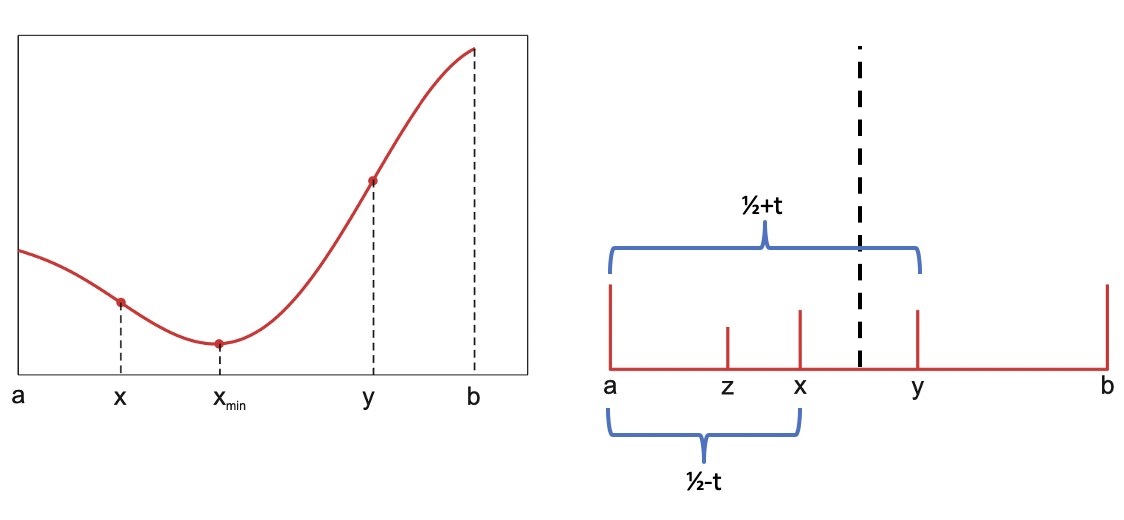
\includegraphics[width=16cm, height=6cm]{images/im221.png}
    \label{ris:im221}
    \caption{Слева: унимодальная функция, справа: точки, выбираемые по золотому сечению}
\end{figure}

\subsubsection{Метод золотого сечения}
В методе золотого сечения точки внутри интервалов поиска решения выбираются исходя из следующих предложений:
\begin{itemize}
    \item на текущей итерации оба потенциальных интервала сокращения равны между собой;
    \item на каждой итерации интервал сокращается на одну и ту же величину.
\end{itemize}
Эти два предложения позволяют однозначно определить процесс генерации новых точек. Предположим, что текущий интервал поиска [a, b] имеет единичную длину и в нём выбраны две точки x, y (см. рисунок \ref{ris:im221}, справа). Равенство потенциальных интервалов сокращения означает, что длина  $[a, x]$ равна $1/2 - t$, а длина $[a, y] - 1/2 + t$, где $t$ – некоторая неизвестная величина.
\newline \newline Пусть на текущей итерации выбирается интервал [a, y] и на следующей итерации к точке x добавляется точка z. Тогда предложение о сокращении интервалов на фиксированную величину означает, что:
$$\dfrac{l[a, y]}{l[a, b]}=\dfrac{l[a, x]}{l[a, y]}=K,$$
где через $l[a, y]$ обозначена длина интервала $[a, y]$. В результате получаем:
$$\dfrac{1/2+t}{1}=\dfrac{1/2-t}{1/2+t} \Rightarrow t = \dfrac{\sqrt{5}-2}{2} \Rightarrow K = \dfrac{\sqrt{5}-1}{2}$$
\newline
\begin{figure}[hbt!]
    \centering
    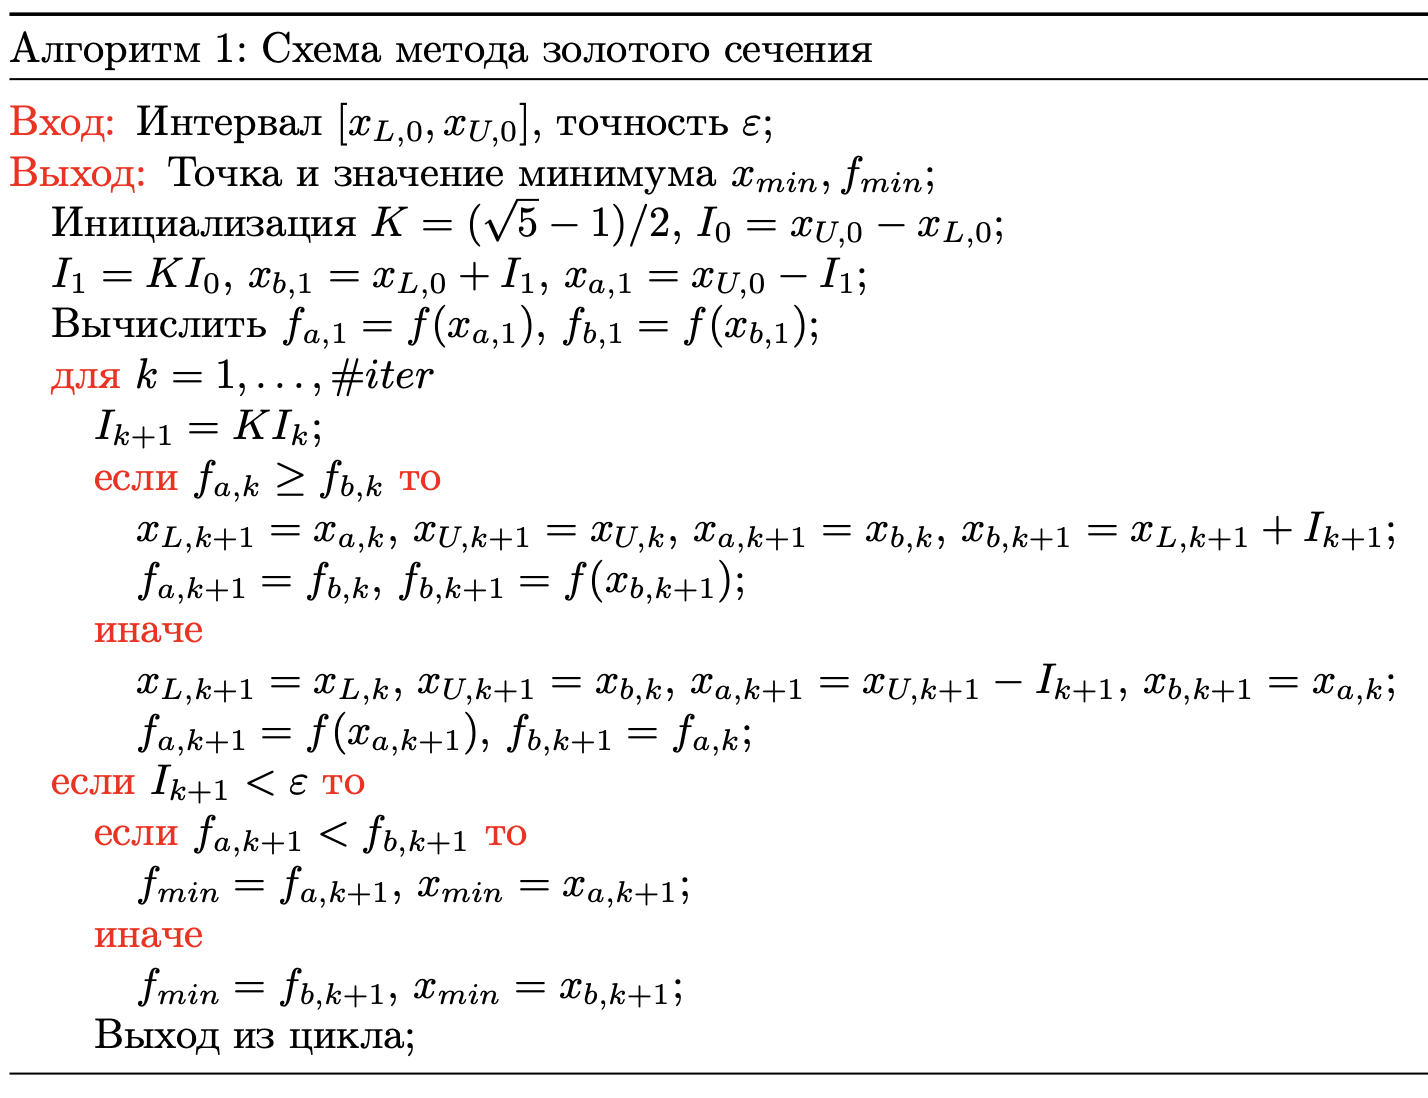
\includegraphics[width=14cm, height=10cm]{images/im222.png}
    \label{ris:im222}
    \caption{Алгоритм 1: Схема метода золотого сечения}
\end{figure}
Схема метода золотого сечения представлена в Алгоритме 1 (см. рисунок \ref{ris:im222}). В этой схеме границы интервала на итерации k обозначены как $x_{L,k}$ и $x_{U,k}$, длина интервала как $I_k$, а две внутренние точки интервала как $x_{a,k}$ и $x_{b,k}$.
Очевидно, что длина интервала $I_k = KI_{k-1} = K^2I_{k-2} = \dots = K^kI_0$, где $I_0$ – длина начального интервала, заданного пользователем. Поэтому \textbf{скорость сходимости} метода золотого сечения является \textbf{линейной} с константой $K$. Кроме того, из условия $ K^kI_0 \textless \varepsilon$  можно определить количество итераций, которые потребуются методу для достижения точности $\varepsilon$. Заметим также, что в методе золотого сечения оптимизируемая функция $f$ \textbf{не вычисляется в крайних точках} $x_{L,0}$ и $x_{U,0}$. Это удобно, например, для оптимизации функций с вертикальными асимптотами.

\subsubsection{Метод парабол}
\begin{figure}[hbt!]
    \centering
    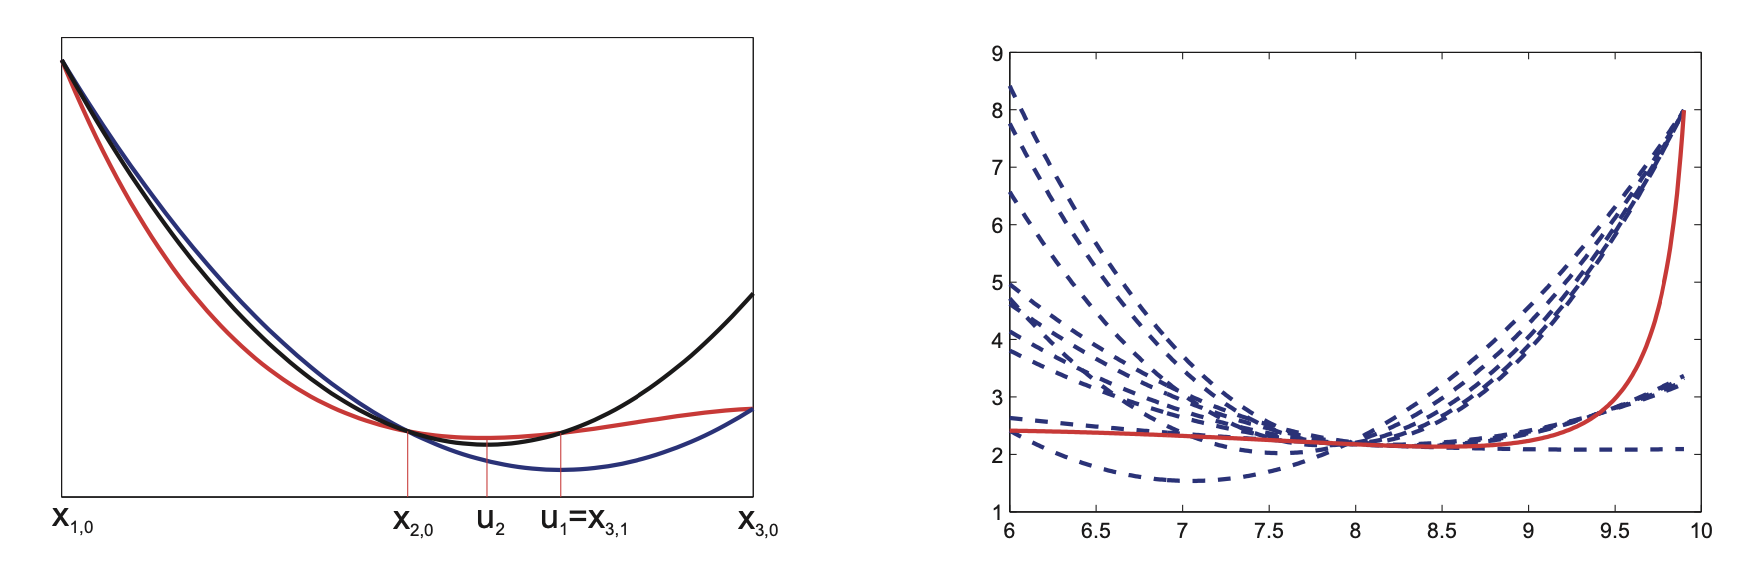
\includegraphics[width=16cm, height=6cm]{images/im223.png}
    \label{ris:im223}
    \caption{ Иллюстрация работы метода парабол. Слева: первые две итерации метода, красная кривая – оптимизируемая функция, синяя кривая – квадратичное приближение на первой итерации, чёрная кривая – квадратичное приближение на второй итерации. Справа: пример плохой сходимости метода парабол, красная кривая – оптимизируемая функция, синие кривые – итерационные квадратичные приближения.}
\end{figure}
В методе парабол предлагается аппроксимировать оптимизируемую функцию $f(x)$ с помощью квадратичной функции:
$$p(x)=ax^2 +bx+c.$$
Пусть имеются три точки $x_1 < x_2 < x_3$ такие, что интервал $[x_1,x_3]$ содержит точку минимума функции $f$. Тогда коэффициенты аппроксимирующей параболы $a, b, c$ могут быть найдены путем решения системы линейных уравнений:
$a x^2_i + bx_i + c = f_i = f ( x_i ) , \ i = 1 , 2 , 3 .$
Минимум такой параболы: $u = -\dfrac{b}{2a}$.
\newline \newline
Если $f(x_2) < f(x_1)$ и $f(x_2) < f(x_3)$, то точка $u$ гарантированно попадает в интервал $[x_1,x_3]$. (см. рисунок \ref{ris:im223}, слева).
\begin{center}
    Если $f(u)\leq f(x_2)$, то $[x_1, x_3] \to [x_1, x_2]$, иначе $[x_1, x_3] \to [u, x_3]$.
\end{center}
В отличие от метода золотого сечения, метод парабол обладает \textbf{суперлинейной скоростью сходимости}. Однако, такая высокая скорость сходимости гарантируется только \textbf{в малой окрестности точки минимума $x_{min}$}. На начальных стадиях процесса оптимизации метод парабол может делать очень маленькие шаги или, наоборот, слишком большие шаги, приводящие к неустойчивым биениям (см. рисунок \ref{ris:im223}, справа). Также следует отметить, что на первой итерации метод парабол \textbf{требует измерения значений функции f в крайних точках} интервала оптимизации.

\subsubsection{Комбинированный метод Брента}
Метод золотого сечения представляет собой надежный способ оптимизации, который сходится за гарантированное число итераций, но обладает лишь линейной скоростью сходимости. Метод парабол работает быстрее в малой окрестности оптимального решения, но может работать долго и неустойчиво на начальных стадиях итерационного процесса. Поэтому на практике для решения задачи одномерной оптимизации используется метод Брента, который эффективно комбинирует эти две стратегии.
\newline \newline В данном методе на каждой итерации отслеживаются значения в шести точках (не обязательно различных): $a, c, x, w, v, u$.
\newline \newline Точки $a, c$ задают текущий интервал поиска решения,
\newline $x$ – точка, соответствующая наименьшему значению функции,
\newline$ w $ – точка, соответствующая второму снизу значению функции,
\newline $v$ – предыдущее значение$ w$.
\newline \newline В отличие от метода парабол, в методе Брента аппроксимирующая парабола строится с помощью трех наилучших точек $x, w, v $(в случае, если эти три точки различны и значения в них также различны). При этом минимум аппроксимирующей параболы $u$ принимается в качестве следующей точки оптимизационного процесса, если:
\begin{itemize}
    \item $u$ попадает внутрь интервала $[a, c]$;
    \item $u$ отстоит от точки $x$ не более, чем на половину от длины предпредыдущего шага.
\end{itemize}
Если точка $u$ отвергается, то следующая точка находится с помощью золотого сечения большего из интервалов $[a, x] $и $[x, c]$. Итоговая схема Брента представлена в Алгоритме 2. (см. рисунок \ref{ris:im224})
\begin{figure}[hbt!]
    \centering
    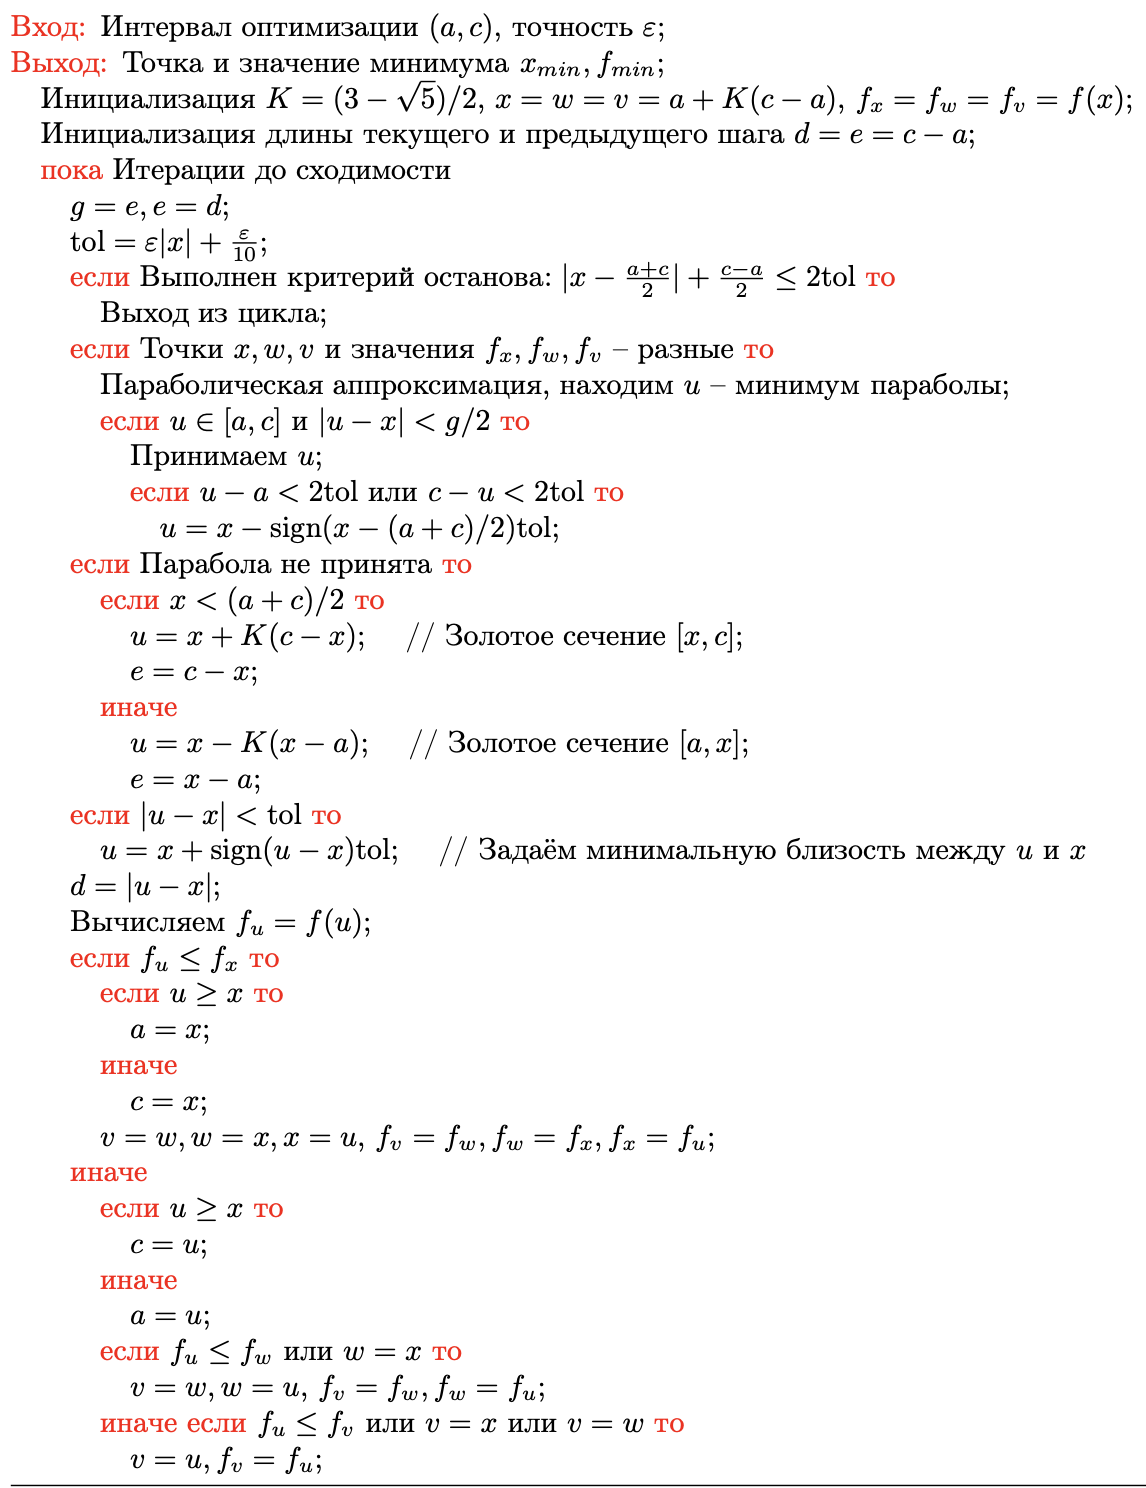
\includegraphics[width=14cm, height=19cm]{images/im224.png}
    \label{ris:im224}
    \caption{Алгоритм 2: Комбинированный метод Брента}
\end{figure}
\newline  \newline
Приведем некоторые аргументы в пользу обозначенных условий приема минимума параболы $u$. Так как парабола на текущей итерации проводится через точки $x,w,v$, для которых не гарантируются соотношения $v < x < w$ или $w < x < v$, то минимум параболы может оказаться вне интервала $[a,c]$. Ограничение на максимальную удалённость $u$ от $x$ позволяет избежать слишком больших шагов в оптимизации, которые могут соответствовать биениям в методе парабол. Использование в данном ограничении длины предпредыдущего шага, а не предыдущего, является эвристикой, эффективность которой подтверждается в экспериментах на больших базах задач оптимизации. Эта эвристика предлагает не штрафовать метод за текущий не слишком удачный маленький шаг в надежде на успешные шаги метода на следующих итерациях.

\subsubsection{Неточная одномерная оптимизация}
Во многих методах многомерной оптимизации на итерации k имеется текущая точка $x_k \in \mathbb{R}^n$ и некоторое направление минимизации $d_k \in \mathbb{R}^n$ . Тогда следующая точка итерационного процесса $x_{k+1}$ находится путем решения следующей задачи одномерной оптимизации:
\begin{equation}
    \label{formula222}
    \phi(\alpha) = f(x_k+\alpha d_k)\to \min_{\alpha \geq 0}.
\end{equation}
Эту задачу можно решать с помощью методов, описанных выше. Однако, для сходимости общего процесса многомерной оптимизации задачу \ref{formula222} зачастую не обязательно решать точно. На практике здесь оказывается достаточным лишь значимо уменьшить значение функции на текущей итерации. Отказ от точного решения  \ref{formula222}  позволяет во многих случаях сократить количество обращений к оракулу.
\newline
Итак, дано:
$$\phi(\alpha) = f(x_k+\alpha d_k)$$
$$\phi'(0) = \nabla f(x_k)^T d_k < 0$$
Условия неточной одномерной оптимизации:
\begin{itemize}
    \item[1.] \textbf{Условие Армихо.}
    Гарантирует уменьшение значения функции на текущей итерации (условие, значимого уменьшения). См. рисунок \ref{ris:im225} слева.
    $$\phi(\alpha_k) \leq \phi(0) + c_1 \alpha_k \phi'(0), c_1 \in (0,1) $$

    \item[2.] \textbf{Условие Вольфа.} Есть два условия - слабое и сильное, мы используем одно из двух. См. рисунок \ref{ris:im225} справа. \newline
    \begin{itemize}
        \item[a.] (слабое условие) $\phi'(\alpha_k)\geq c_2 \ \phi'(0), \ c_2 \in (0,1)$
        \item[b.] (сильное условие) $|\phi(\alpha_k)|\leq c_2 \ |\phi'(0)|, \ c_2 \in (0,1)$
    \end{itemize}
    Сильное условие Вольфа позволяет эффективно локализовывать минимум: если константу $c_2$ начинаем стремить к 0, мы все сильнее сжимаем интервал (на рис. между голубой и красной точками) и гарантируем то, что $\alpha_k$, удовлетворяющая сильному условию, будет приблеженным точным оптимумом при $c_2 \to 0$.
    \begin{figure}[hbt!]
        \centering
        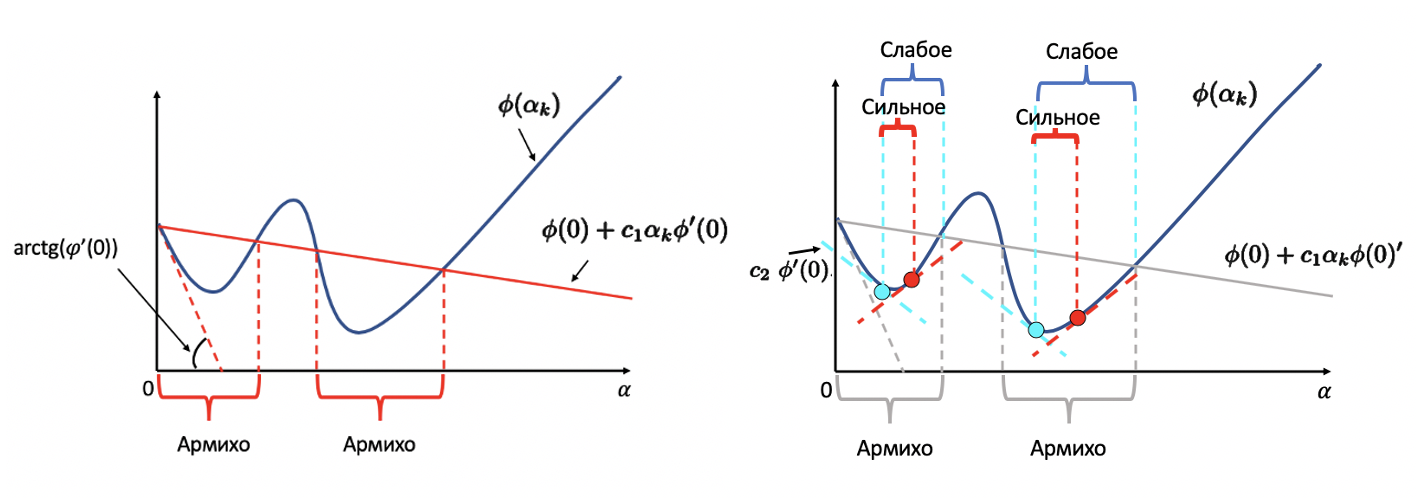
\includegraphics[width=16cm, height=6cm]{images/im225.png}
        \caption{Иллюстрация достаточных условий для неточной одномерной минимизации. Слева: условие Армихо, справа: слабое/сильное условие Вольфа.}
        \label{ris:im225}
    \end{figure}
    \newline
    На практике берут $c_1=10^{-4}, \ c_2 = 0.9$ (если интересует незначительное уменьшение функции) или $c_2=0.1$ (если важно посильнее минимизировать функцию)
\end{itemize}
\textbf{Теорема.}
Если $\phi(\alpha)\in C^1, \ \phi'(\alpha)<0, \phi(\alpha)>-\infty \ \forall \alpha$ и
$0<c_1\leq c_2<1 \Rightarrow$ \newline
$\exists \alpha_*,$ удовлетворяющая условию Армихо и слабому или сильному условию Вольфа.
\newline \textbf{Доказательство.}
$$\phi(\alpha)=\phi(0)+\phi'(0) \alpha + o(\alpha^2) \leq \phi(0)+c_1\alpha\phi'(0)$$
$$\phi'(0)+o(\alpha)\leq c_1 \phi'(0)$$
$$\underbrace{\underbrace{(1 -c_1)}_{\text{>0}}\underbrace{\phi'(0)}_{\text{<0}}}_{\text{<0}}+o(\alpha)\leq 0$$
\begin{center}
    $=> \exists \alpha_*: \forall \alpha \in (0, \alpha_*)$
    условие Армихо выполнено.
\end{center}
$$\exists \hat{\alpha} \ : \ \phi(\hat{\alpha})=\phi(0)+c_1 \hat{\alpha}  \phi'(0)$$
$$\psi(\alpha) := \phi(\alpha)-\phi(0)-c_1\alpha\phi'(0) $$
\begin{center}
    $\psi(0)=0; \ \psi(\hat{\alpha})=0$
    и т. к. $\alpha_*$ лежит между 0 и $\hat{\alpha} => \exists \alpha_* : \ \psi'(\alpha_*)=0$
\end{center}
$$\psi'(\alpha_*)=\phi'(\alpha_*)-c_1 \phi'(0)=0 $$
$$=> \ \phi'(\alpha_*)=c_1 \underbrace{\phi'(0)}_{<0} \geq c_2 \phi'(0)$$
\begin{center}
    $=> \ \alpha_*$ удовлетворяет слабому условию Вольфа.
\end{center}
$$|\phi'(\alpha_*)|=|c_1\phi'(0)|\leq c_2 |\phi'(0)|$$
\begin{center}
    $=> \ \alpha_*$ удовлетворяет сильному условию Вольфа.
\end{center}
\hfill$\scriptstyle\blacksquare$
\textbf{Алгоритм поиска $\alpha_*$.}
\begin{itemize}
    \item[1.] \textbf{Расширение (поиск правой границы)} \\
    Пользователь задает начальную точку $\alpha_0$. Сначала нужно найти интервал, в котором находится искомая точка, т.е. берется точка $\alpha_0$ и умножается на некоторую константу (сдвигается вправо) пока не будет выполнено одно из условий для правой границы.
    \item[2.] \textbf{Сужение} \\
    Теперь интервал нужно сужать:
    \begin{itemize}
        \item[i.] Внутри текущего интервала генерируем (через метод парабол или золотого сечения) какую-то точку
        \item[ii.] Проверяем для нее условия Армихо и Вольфа, если они не выполнены, то сдвигаем интервал налево или направо по условиям для правой и левой границ.
        \item[iii.] Сужаем интервал пока не найдем нужную точку.
    \end{itemize}
\end{itemize}
\textbf{ Условия для правой границы:}
\begin{itemize}
    \item[1.] Не выполнено условие Армихо
    \item[2.] $\phi'(\alpha)>0$ и не выполнено условие Вольфа
    \item[3.] $\phi(\alpha)>\phi(\alpha_{prev})$
\end{itemize}
\textbf{ Условие для левой границы:} в левой точке $\phi'(\alpha)<0$